%
% $Id: $
%
%
% Compilar a .pdf con LaTeX (pdflatex)
% Es necesario instalar Beamer (paquete latex-beamer en Debian)
%

%
% Gr�ficos:
% Los gr�ficos pueden suministrarse en PNG, JPG, TIF, PDF, MPS
% Los EPS deben convertirse a PDF (usar epstopdf)
%

\documentclass{beamer}
\usetheme{Warsaw}
%\usebackgroundtemplate{
\includegraphics[width=\paperwidth]{format/libresoft-bg.png}}
%\usepackage[spanish]{babel}
\usepackage[latin1]{inputenc}
\usepackage{graphics}
\usepackage{amssymb} % Simbolos matematicos
\usepackage{url}

\addtobeamertemplate{navigation symbols}{}{%
    \usebeamerfont{footline}%
    \usebeamercolor[fg]{footline}%
    \hspace{1em}%
    \insertframenumber/\inserttotalframenumber
}



%\definecolor{libresoftgreen}{RGB}{162,190,43}
%\definecolor{libresoftblue}{RGB}{0,98,143}

%\setbeamercolor{titlelike}{bg=libresoftgreen}

%% Metadatos del PDF.
\hypersetup{
  pdftitle={},
  pdfauthor={Jes�s Moreno Le�n, Gregorio Robles},
  pdfcreator={GSyC/LibreSoft \\ Universidad Rey Juan Carlos},
  pdfproducer=PDFLaTeX,
  pdfsubject={Code smells, Computational Thinking, Automatic assessment with Dr. Scratch},
}
%%

\begin{document}

\title[Default names in Scratch]{Hackathon: use of default names in Scratch projects (SpriteX)}
\institute{jesus.moreno@programamos.es, grex@gsyc.urjc.es \\
GSyC/Libresoft, Universidad Rey Juan Carlos}
\author[J. Moreno-Le�n, G. Robles]{Jes�s Moreno-Le�n, Gregorio Robles}
\date{SATToSE, Madrid, June 9\textsuperscript{th}, 2017}

\frame{
\maketitle
\begin{center}

\includegraphics[width=2cm]{format/libresoft-logo}
\hspace{0.5cm}

\includegraphics[width=5cm]{format/gsyc-urjc}
%\vspace{0.5cm}

\includegraphics[width=3cm]{format/emadrid.png}
\end{center}
}


% Si el titulo o el autor se quieren acortar para los pies de p�gina
% se pueden redefinir aqu�:
% \title{Present and Future of Dr. Scratch}
% \author{J. Moreno-Le�n, G. Robles \& M. Rom\'an-Gonz\'alez}

%% LICENCIA DE REDISTRIBUCION DE LAS TRANSPAS
\frame{
~
\vspace{3cm}

\begin{flushright}

\includegraphics[width=2.2cm]{figs/by-sa}
\vspace{0.4cm}
{\tiny
(cc) 2017 Jes�s Moreno Le�n and Gregorio Robles \\
  Some rights reserved. This work licensed under Creative Commons \\
  Attribution-ShareAlike License. To view a copy of full license, see \\
  http://creativecommons.org/licenses/by-sa/3.0/ or write to \\
  Creative Commons, 559 Nathan Abbott Way, Stanford, \\
  California 94305, USA. \\
\ \\
Some of the figures have been taken from the Internet \\
Source, and author and licence if known, is specified. \\
For those images, \emph{fair use} applies.\\
%A copy of this document is available at\\ https://www.slideshare.net/jmorenol/can-we-measure-computational-thinking-with-tools-present-and-future-of-dr-scratch
}
\end{flushright}
}
%%

\section{SATToSE 17, Madrid}


%--------------------------------------------------------
%\usebackgroundtemplate{
\includegraphics[width=10cm]{figs/drscratch1}}

\begin{frame}
\frametitle{Default names in Scratch}

\begin{figure}[t!]
\begin{center}
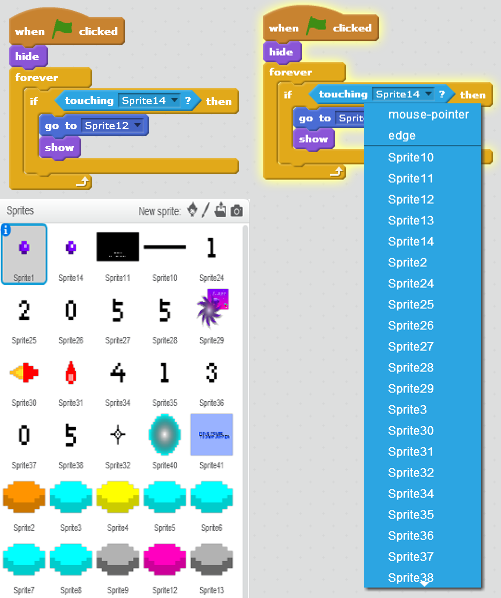
\includegraphics[width=7cm, height=6cm]{figs/SpriteNaming.png}
\end{center}
\label{fig:naming}
\end{figure}

\end{frame}

%--------------------------------------------------------

%\usebackgroundtemplate{
\includegraphics[width=10cm]{figs/drscratch1}}

\begin{frame}
\frametitle{Is this smell common in the Scratch repository?}

\begin{figure}[t!]
\begin{center}
\begin{center}
%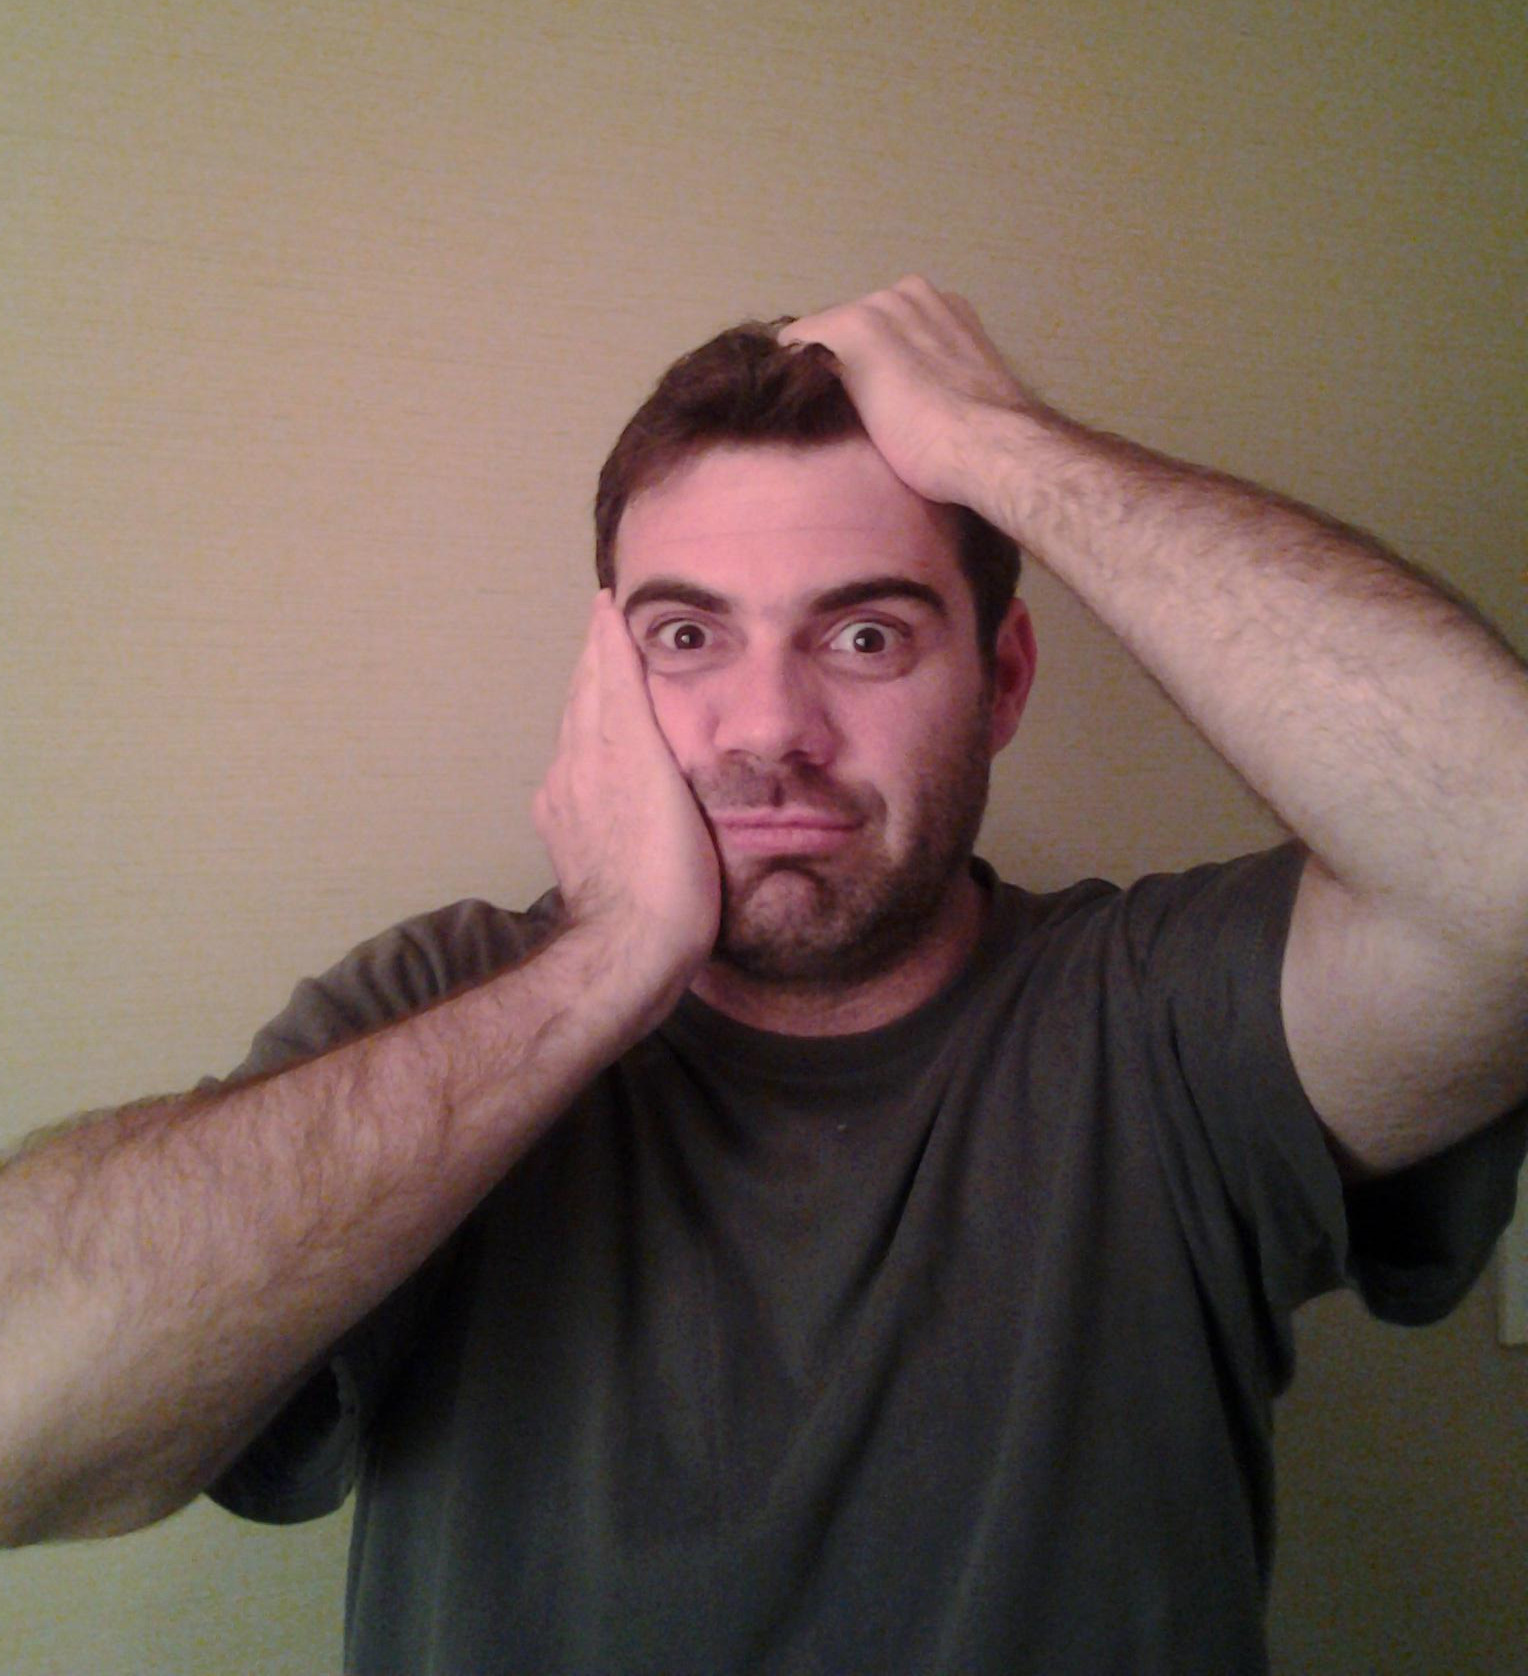
\includegraphics[width=6cm]{figs/face.jpg}
\end{center}
\huge 53.4\% of projects in the dataset contain sprites with default names
\end{center}
\label{fig:naming}
\end{figure}

\end{frame}

%--------------------------------------------------------
%\usebackgroundtemplate{
\includegraphics[width=10cm]{figs/drscratch1}}

\begin{frame}
\frametitle{Do advanced programmers avoid using default names? (I)}

\begin{figure}[t!]
\begin{center}
\includegraphics[width=8cm]{figs/ByScore.png}
\end{center}
\end{figure}

\end{frame}

%--------------------------------------------------------

%\usebackgroundtemplate{
\includegraphics[width=10cm]{figs/drscratch1}}

\begin{frame}
\frametitle{Do advanced programmers avoid using default names? (II)}

\begin{figure}[t!]
\begin{center}
\includegraphics[width=8cm]{figs/ByAspect.png}
\end{center}
\end{figure}

\end{frame}

%--------------------------------------------------------

%\usebackgroundtemplate{
\includegraphics[width=10cm]{figs/drscratch1}}

\begin{frame}
\frametitle{Do advanced programmers avoid using default names? (III)}
\begin{center}
\begin{table}[]
\centering
\label{table:levels}
\begin{tabular}{ccc}
Level & Mastery score & \% sprites w/ default names \\ \hline
Basic & 0-7 & .50 \\
Intermediate & 8-14 & .35 \\
Advanced & 15-21 & .28 \\ \hline
\end{tabular}
\caption{Differences in the use of default names in terms of mastery score}
\end{table}
\end{center}

\end{frame}

%--------------------------------------------------------
\frame{
\maketitle
\begin{center}

\includegraphics[width=2cm]{format/libresoft-logo}
\hspace{0.5cm}

\includegraphics[width=5cm]{format/gsyc-urjc}
\vspace{0.5cm}

\includegraphics[width=3cm]{format/emadrid.png}
\end{center}
}

\end{document}
